\حصہ{تکونیاتی تفاعل کا تفرق}
بہت سارے طبعی اعمال، مثلاً برقناطیسی امواج، دل کی دھڑکن، موسم، وغیرہ، دوری ہوتے ہیں۔ اعلٰی احصاء کا ایک مسئلہ کہتا ہے کہ ہر دوری تفاعل جو ہم حقیقت میں استعمال ہوتا ہو کو سائن اور کوسائن تفاعل کا مجموعہ لکھا جا سکتا ہے۔یوں تبدیلی پر غور کرنے میں سائن اور کوسائن تفاعل اہم کردار ادا کرتے ہیں۔اس حصے میں چھ تکونیاتی تفاعل کا تفرق کرنا سکھایا جائے گا۔

\جزوحصہء{چند اہم حد} 
ہم سب سے پہلے چند عدم مساوات اور حد پیش کرتے ہیں۔ زاویوں کی پیمائش ریڈیئن میں ہے۔

\ابتدا{مسئلہ}\شناخت{مسئلہ_تفرق_سائن_زاویہ_سے_کم}
اگر \عددی{\theta} کی پیمائش ریڈیئن میں ہو تب درج ذیل ہوں گے۔
\begin{align*}
-\abs{\theta}<\sin\theta \abs{\theta} \quad \text{اور}\quad -\abs{\theta}<1-\cos\theta<\abs{\theta}
\end{align*}
\انتہا{مسئلہ}
%==========================
 \ابتدا{ثبوت}
ان عدم مساوات کو ثابت کرنے کے لئے ہم  شکل \حوالہ{شکل_تفرق-تکونیاتی_تعلق} پر غور کرتے ہیں جہاں \عددی{\theta} ربع اول میں واقع ہے لہٰذا اکائی دائرے کے قوس \عددی{NA} کی لمبائی \عددی{\abs{\theta}} ہو گی۔چونکہ (سیدھی) قطع  \عددی{AN} کی لمبائی قوس \عددی{AN} کی لمبائی \عددی{\theta} سے کم ہے لہٰذا قائمہ مثلث \عددی{ANQ} میں مسئلہ فیثاغورث کی مدد سے
\begin{align*}
\sin^2\theta+(1-\cos\theta)^2=(AN)^2<\theta^2
\end{align*}
لکھا جا سکتا ہے۔چونکہ مربع کی قیمت مثبت ہوتی ہے لہٰذا بائیں طرف دونوں اجزاء مثبت ہیں۔ دو مثبت قیمتوں کا مجموعہ دونوں کے انفرادی قیمت سے زیادہ ہوتی ہے لہٰذا
\begin{align*}
\sin^2\theta<\theta^2,\quad (1-\cos\theta)^2<\theta^2
\end{align*}
لکھے جا سکتے ہیں جن کا جذر لینے سے
\begin{align*}
\abs{\sin\theta}<\abs{\theta},\quad \abs{1-\cos\theta}<\abs{\theta}
\end{align*}
یعنی
\begin{align*}
-\abs{\theta}<\sin\theta<\abs{\theta},\quad -\abs{\theta}<1-\cos\theta<\abs{\theta}
\end{align*}
حاصل ہوتے ہیں۔
\begin{figure}
\centering
\begin{tikzpicture}
\pgfmathsetmacro{\r}{2.2}
\pgfmathsetmacro{\ang}{60}
\draw[-latex](-\r-0.5,0)--(\r+1.5,0)node[right]{$x$};
\draw[-latex](0,-0.25)--(0,\r+0.5)node[above]{$y$};
\draw([shift={(-10:\r)}]0,0) arc (-10:190:\r);
\draw(0,0)node[below left]{$(0,0)$}--(\ang:\r)coordinate(kA)node[above]{$N$}node[pos=0.4,above left]{$1$}--(\r,0)node[below right]{$A(1,0)$};
\draw[-latex]([shift={(0:0.5)}]0,0) arc (0:\ang:0.5);
\draw(\ang/2:0.7)node[]{$\theta$};
\draw[thick](kA)--($(0,0)!(kA)!(\r,0)$)coordinate(kB)node[below]{$Q$}node[pos=0.6,rotate=-90,above]{$\sin \theta$}--(0,0)node[pos=0.5,below]{$\cos \theta$};
\draw[thick] ([shift={(0:\r)}]0,0) arc (0:\ang:\r);
\draw(25:\r+0.3)node[]{$\theta$};
\RightAngle{(kA)}{(kB)}{(0,0)}
\draw[decoration={brace,mirror,raise=5pt},decorate](kB)++(0,-0.4) -- (\r,-0.4)node[midway,below,yshift=-2mm]{$1-\cos\theta$};
\end{tikzpicture}
\caption{اس شکل کی جیومیٹری، جس میں \عددی{\theta>0} ہے، سے عدم مساوات \عددی{\sin^2\theta+(1-\cos\theta)^2<\theta^2} لکھی جا سکتی ہے۔}
\label{شکل_تفرق-تکونیاتی_تعلق}
\end{figure}
\انتہا{ثبوت}
%==============================

\ابتدا{مثال}
دکھائیں کہ \عددی{\theta=0} پر \عددی{\sin\theta} اور \عددی{\cos\theta} استمراری ہیں یعنی:
\begin{align*}
\lim_{\theta\to 0} \sin\theta=0,\quad \lim_{\theta \to 0} \cos \theta=1
\end{align*}
حل:\quad
\عددی{\theta\to 0} کرنے سے \عددی{\abs{\theta}} اور \عددی{-\abs{\theta}} دونوں صفر کے نزدیک تر ہوتے ہیں۔یوں مسئلہ \حوالہ{مسئلہ_تفرق_سائن_زاویہ_سے_کم} اور مسئلہ  بیچ سے مذکورہ بالا حد ثابت ہوتے ہیں۔
\انتہا{مثال}
%================================

تفاعل \عددی{f(\theta)=\tfrac{\sin\theta}{\theta}} جہاں \عددی{\theta} کی پیمائش ریڈیئن میں ہے کو شکل \حوالہ{شکل_تفرق_سنک_تفاعل} میں ترسیم کیا گیا ہے جس کو دیکھ کر ایسا معلوم ہوتا ہے جیسے \عددی{\theta=0} پر قابل ہٹاو عدم استمرار پایا جاتا ہے۔اس شکل کے مطابق \عددی{\lim\limits_{\theta\to 0}f(\theta)=1} ہو گا۔
\begin{figure}
\centering
\begin{minipage}{0.45\textwidth}
\centering
\begin{tikzpicture}
\begin{axis}[small,axis lines=middle,xlabel={$\theta$},ylabel={$y$},xtick={-9.426,-6.284,-3.142,3.142,6.284,9.426},xticklabels={$-3\pi$,$-2\pi$,$-\pi$,$\pi$,$2\pi$,$3\pi$},ytick={1},xmax=11,ymax=1.25,xlabel style={at={(current axis.right of origin)},anchor=west}]
\addplot[domain=-10:10,samples=100]{sin(deg(x))/x};
\draw(axis cs:0,1)node[circ]{};
\draw(axis cs:3.142,0.75)node[right]{$y=\frac{\sin\theta}{\theta}$};
\end{axis}
\end{tikzpicture}
\caption{تفاعل \عددی{f(\theta)=\tfrac{\sin\theta}{\theta}} جہاں \عددی{\theta} کی پیمائش ریڈیئن میں ہے۔}
\label{شکل_تفرق_سنک_تفاعل}
\end{minipage}\hfill
\begin{minipage}{0.45\textwidth}
\centering
\begin{tikzpicture}
\pgfmathsetmacro{\r}{2.5}
\pgfmathsetmacro{\ang}{45}
\pgfmathsetmacro{\ky}{\r/cos(\ang)}
\draw[-latex](0-0.25,0)--(\r+1,0)node[right]{$x$};
\draw[-latex](0,-0.2)--(0,\r+0.5)node[above]{$y$};
\draw([shift={(0:\r)}]0,0) arc (0:90:\r);
\draw[-stealth]([shift={(0:0.5)}]0,0) arc (0:\ang:0.5);
\draw(\ang/2:0.7)node[]{$\theta$};
\draw(0,0)node[below left]{$M$}--++(\ang:\ky)node[pos=0.4,above left]{$1$}node[right]{$T$}--(\r,0)node[below,xshift={2mm}]{$A(1,0)$}node[pos=0.5,right]{$\tan\theta$};
\draw(\ang:\r)coordinate(kA)node[above]{$N$}--(\r,0);
\draw[thick](kA)--($(0,0)!(kA)!(\r,0)$)coordinate(kB)node[below]{$Q$}node[pos=0.6,left]{$\sin\theta$}--(0,0)node[pos=0.5,below]{$\cos\theta$};
\RightAngle{(kA)}{(kB)}{(0,0)}
\draw(0,1)node[left]{$1$};
\end{tikzpicture}
\caption{برائے مسئلہ \حوالہ{مسئلہ_تفرق_سائن_بٹا_زاویہ}}
\label{شکل_مسئلہ_تفرق_سائن_بٹا_زاویہ}
\end{minipage}%
\end{figure}

\ابتدا{مسئلہ}\شناخت{مسئلہ_تفرق_سائن_بٹا_زاویہ}
\begin{align}
\lim_{\theta\to 0} \frac{\sin\theta}{\theta}=1\quad\quad \text{(\RL{\عددی{\theta} کی پیمائش ریڈیئن میں ہے})}
\end{align}
\انتہا{مسئلہ}
%===============================
\ابتدا{ثبوت}
ہم بائیں ہاتھ حد اور دائیں ہاتھ حد کو \عددی{1} کے برابر ثابت کرتے ہیں۔یوں دو طرفہ حد بھی \عددی{1} ہو گا۔ 

دائیں ہاتھ حد کو \عددی{1} کے برابر ثابت کرنے کی خاطر ہم \عددی{\theta} کی قیمت مثبت اور \عددی{\tfrac{\pi}{2}} سے کم رکھتے ہیں (شکل \حوالہ{شکل_مسئلہ_تفرق_سائن_بٹا_زاویہ})۔ آپ دیکھ سکتے ہیں کہ
\begin{align*}
\Delta MAN \text{رقبہ}<MAN \text{\RL{رقبہ خطہ}}<\Delta MAT \text{رقبہ}
\end{align*}
ہے۔ان رقبوں کو \عددی{\theta} کی صورت
\begin{align*}
\Delta MAN\text{رقبہ}&=\frac{1}{2}\times \text{قاعدہ}\times \text{عمود}=\frac{1}{2}(1)(\sin\theta)=\frac{1}{2}\sin\theta\\
MAN\text{\RL{رقبہ خطہ}}&=\frac{1}{2}r^2\theta=\frac{1}{2}(1)^2\theta=\frac{\theta}{2}\\
\Delta MAT\text{رقبہ}&=\frac{1}{2}\times\text{قاعدہ}\times\text{عمود}=\frac{1}{2}(1)(\tan\theta)=\frac{1}{2}\tan\theta
\end{align*}
میں لکھتے ہوئے درج ذیل تعلق حاصل ہوتا ہے
\begin{align*}
\frac{1}{2}\sin\theta<\frac{1}{2}\theta<\frac{1}{2}\tan\theta
\end{align*}
جس کو \عددی{\tfrac{1}{2}\sin\theta} سے تقسیم کرنے سے
\begin{align*}
1<\frac{\theta}{\sin\theta}<\frac{1}{\cos\theta}
\end{align*}
حاصل ہو گا۔اس کا بالعکس متناسب لیتے ہیں جس سے عدم مساوات کی علامتیں الٹ ہوتی ہیں۔
\begin{align*}
1>\frac{\sin\theta}{\theta}>\cos\theta
\end{align*}
چونکہ \عددی{\lim_{\theta\to 0^+}\cos\theta=1} ہے لہٰذا مسئلہ بیچ کے تحت درج ذیل ہو گا۔
\begin{align*}
\lim_{\theta\to 0^+}\frac{\sin\theta}{\theta}=1
\end{align*}
آخر میں دھیان رہے کہ \عددی{\sin\theta} اور \عددی{\theta} دونوں \ترچھا{طاق تفاعل} ہیں لہٰذا \عددی{f(\theta)=\tfrac{\sin\theta}{\theta}} \ترچھا{جفت تفاعل} ہو گا جس کا ترسیم \عددی{y} محور کے دونوں اطراف یکساں ہو گا (شکل \حوالہ{شکل_تفرق_سنک_تفاعل})۔اس تشاکلی کی بنا بائیں ہاتھ حد بھی موجود ہو گا اور اس کی قیمت بھی \عددی{1} ہو گی۔
\begin{align*}
\lim_{\theta\to 0^-}\frac{\sin\theta}{\theta}=1=\lim_{\theta\to 0^+}\frac{\sin\theta}{\theta}
\end{align*}
یوں صفحہ \حوالہصفحہ{مسئلہ_حد_یک_طرفہ_بالمقابل_دو_طرفہ_حد} پر مسئلہ \حوالہ{مسئلہ_حد_یک_طرفہ_بالمقابل_دو_طرفہ_حد} کے تحت \عددی{\lim_{\theta\to 0}\tfrac{\sin\theta}{\theta}=1} ہو گا۔
\انتہا{ثبوت}
%===================================

مسئلہ \حوالہ{مسئلہ_تفرق_سائن_بٹا_زاویہ} کو قواعد حد اور معلوم تکونیاتی مماثل کے ساتھ ملاتے ہوئے دیگر تکونیاتی حد تلاش کیے جا سکتے ہیں۔ 

\ابتدا{مثال}\شناخت{مثال_تفرق_سائن_الف}
دکھائیں کہ \عددی{\lim_{h\to 0}\tfrac{\cos h-1}{h}=0} ہے۔\\
حل:\quad
نصف زاویہ کلیہ استعمال کرتے ہوئے \عددی{\cos h=1-2\sin^2\tfrac{h}{2}} لکھتے ہوئے درج ذیل ہو گا۔
\begin{align*}
\lim_{h\to 0}\frac{\cos h-1}{h}&=\lim_{h\to 0}-\frac{2\sin^2\tfrac{h}{2}}{h}\\
&=-\lim_{\theta\to 0} \frac{\sin\theta}{\theta}\sin\theta\quad\quad (\theta=\frac{h}{2})\\
&=-(1)(0)=0
\end{align*}
\انتہا{مثال}
%===========================

\جزوحصہء{سائن تفاعل کا تفرق}
تفاعل \عددی{y=\sin\theta} کا تفرق جاننے کی خاطر ہم مثال \حوالہ{مثال_تفرق_سائن_الف} کے حد اور  مسئلہ \حوالہ{مسئلہ_تفرق_سائن_بٹا_زاویہ} کو  کلیہ 
\begin{align*}
\sin(x+h)=\sin x\cos h+\cos x\sin h
\end{align*}
کے ساتھ ملا کر حل کرتے ہیں۔
\begin{align*}
\frac{\dif y}{\dif x}&=\lim_{h\to 0}\frac{\sin(x+h)-\sin x}{h}\\
&=\lim_{h\to 0} \frac{(\sin x\cos h+\cos x\sin h)-\sin x}{h}\\
&=\lim_{h\to 0} \frac{\sin x(\cos h-1)+\cos x\sin h}{h}\\
&=\lim_{h\to 0} \big(\sin x\cdot \frac{\cos h-1}{h}\big)+\lim_{h\to 0}\big(\cos x\cdot \frac{\sin h}{h}\big)\\
&=\sin x\cdot \lim_{h\to 0}\frac{\cos h-1}{h}+\cos x\cdot \lim_{h\to 0}\frac{\sin h}{h}\\
&=\sin x\cdot 0+\cos x \cdot 1\\
&=\cos x
\end{align*}
یوں سائن تفاعل کا تفرق کوسائن تفاعل ہے۔
\begin{align*}
\frac{\dif}{\dif x} (\sin x)=\cos x
\end{align*}

\ابتدا{مثال}
\begin{enumerate}[a.]
\item
\begin{gather*}
\begin{aligned}[t]
y=x^2-\sin x:
\end{aligned}
\quad
\begin{aligned}[t]
\frac{\dif y}{\dif x}&=2x-\frac{\dif}{\dif x}(\sin x) \quad (\text{\RL{قاعدہ فرق}})\\
&=2x-\cos x
\end{aligned}
\end{gather*}
\item
\begin{gather*}
\begin{aligned}[t]
y=x^2\sin x:
\end{aligned}\quad
\begin{aligned}[t]
\frac{\dif y}{\dif x}&=x^2\frac{\dif}{\dif x}(\sin x)+2x\sin x\quad (\text{\RL{قاعدہ حاصل ضرب}})\\
&=x^2\cos x+2x\sin x
\end{aligned}
\end{gather*}
\item
\begin{gather*}
\begin{aligned}[t]
y=\frac{\sin x}{x}:
\end{aligned}\quad
\begin{aligned}[t]
\frac{\dif y}{\dif x}&=\frac{x\cdot \tfrac{\dif}{\dif x}(\sin x)-\sin x\cdot 1}{x^2}\quad \text{\RL{قاعدہ حاصل تقسیم}}\\
&=\frac{x\cos x-\sin x}{x^2}
\end{aligned}
\end{gather*}
\end{enumerate}
\انتہا{مثال}
%=========================

آپ نے دیکھا کہ اگر زاویہ کی پیمائش ریڈیئن میں ہو تب \عددی{\lim_{\theta \to 0}\tfrac{\sin\theta}{\theta}=1} ہوتا ہے اور \عددی{\sin x} کا تفرق
 \عددی{\cos x} ہوتا ہے۔یہی وجہ ہے کہ احصاء کی میدان میں زاویہ کو درجات کی بجائے ریڈیئن میں ناپا جاتا ہے۔

\جزوحصہء{کوسائن کا تفرق}
کوسائن کا تفرق حاصل کرنے کی خاطر ہمیں کلیہ
\begin{align*}
\cos(x+h)=\cos x\cos h-\sin x\sin h
\end{align*}
استعمال کرنا ہو گا۔
\begin{align*}
\frac{\dif y}{\dif x}(\cos x)&=\lim_{h\to 0}\frac{\cos(x+h)-\cos x}{h}\quad\text{(\RL{تفرق کی تعریف})}\\
&=\lim_{h\to 0}\frac{(\cos x\cos h-\sin x\sin h)-\cos x}{h}\\
&=\lim_{g\to 0}\frac{\cos x(\cos h-1)-\sin x\sin h}{h}\\
&=\lim_{h\to 0}\cos x\cdot \frac{\cos h-1}{h}-\lim_{h\to 0}\sin x\cdot \frac{\sin h}{h}\\
&=\cos x\cdot \lim_{h\to 0}\frac{\cos h-1}{h}-\sin x\cdot \lim_{h\to 0}\frac{\sin h}{h}\\
&=\cos x\cdot 0-\sin x\cdot 1\quad\quad \quad \text{(\RL{مثال \حوالہ{مثال_تفرق_سائن_الف} اور مسئلہ \حوالہ{مسئلہ_تفرق_سائن_بٹا_زاویہ}})}\\
&=-\sin x
\end{align*}
یوں کوسائن کا تفرق منفی سائن ہو گا۔
\begin{align*}
\frac{\dif}{\dif x}(\cos x)=-\sin x
\end{align*}

درج بالا تعلق کو شکل \حوالہ{شکل_تفرق_کوسائن_کا_تفرق_سائن} میں دکھایا گیا ہے۔آپ دیکھ سکتے ہیں کہ جہاں کوسائن تفاعل کی ڈھلوان صفر ہے (یعنی \عددی{x=-\pi,0,\pi}) وہاں اس کا تفرق یعنی \عددی{y'=-\sin x} کی قیمت صفر ہے۔اسی طرح جہاں کوسائن تفاعل کی ڈھلوان زیادہ سے زیادہ  بڑھتی یا گھٹتی ہے (مثلاً بالترتیب \عددی{x=-\tfrac{\pi}{2}} اور \عددی{x=\tfrac{\pi}{2}} پر) وہاں اس کے تفرق کی  (بالترتیب مثبت اور منفی) چوٹی پائی جاتی ہے۔
\begin{figure}
\centering
\begin{tikzpicture}
\begin{axis}[clip=false,small,axis lines=middle,ymin=-1.25,ymax=1.5,ytick={-1,1},xtick={-3.142,3.142,-1.571,1.571},xticklabels={$-\pi$,$\pi$,$-\tfrac{\pi}{2}$,$\tfrac{\pi}{2}$},xmax=5.5,xlabel={$x$},ylabel={$y$},xlabel style={at={(current axis.right of origin)},anchor=west}]
\addplot[domain=-5:5,samples=100]{-sin(deg(x))}node[right]{$y'=-\sin x$};
\addplot[domain=-5:5,samples=100]{cos(deg(x))}node[right]{$y=\cos x$};
\draw(axis cs:-0.5,1)--(axis cs:0.5,1)  (axis cs:3.142-0.5,-1)--(axis cs:3.142+0.5,-1)  (axis cs:-3.142-0.5,-1)--(axis cs:-3.142+0.5,-1);
\end{axis}
\end{tikzpicture}
\caption{تفاعل \عددی{y=\cos x} کی ڈھلوان تفاعل \عددی{y'=-\sin x} دیتی ہے۔}
\label{شکل_تفرق_کوسائن_کا_تفرق_سائن}
\end{figure} 

\ابتدا{مثال}
\begin{enumerate}[a.]
\item
\begin{align*}
y&=5x+\cos x\\
\frac{\dif y}{\dif x}&=\frac{\dif}{\dif x}(5x)+\frac{\dif}{\dif x}(\cos x)\\
&=5-\sin x
\end{align*}
\item
\begin{align*}
y&=\sin x\cos x\\
\frac{\dif y}{\dif x}&=\sin x\frac{\dif}{\dif x}(\cos x)+\cos x\frac{\dif}{\dif x}(\sin x)\quad \text{(\RL{قاعدہ حاصل ضرب})}\\
&=\sin x(-\sin x)+\cos x(\cos x)\\
&=\cos^2x-\sin^2x
\end{align*}
\item
\begin{align*}
y&=\frac{\cos x}{1-\sin x}\\
\frac{\dif y}{\dif x}&=\frac{(1-\sin x)\tfrac{\dif}{\dif x}(\cos x)-\cos x\tfrac{\dif}{\dif x}(1-\sin x)}{(1-\sin x)^2}\quad \text{(\RL{قاعدہ حاصل تقسیم})}\\
&=\frac{(1-\sin x)(-\sin x)-\cos x(0-\cos x)}{(1-\sin x)^2}\\
&=\frac{1-\sin x}{(1-\sin x)^2}\quad\quad\quad\quad\quad (\sin^2x+\cos^2x=1)\\
&=\frac{1}{1-\sin x}
\end{align*}
\end{enumerate}
\انتہا{مثال}
%============================

\جزوحصہء{سادہ ہارمونی حرکت}
ایک  اسپرنگ سے  لٹکائے گئے جسم کو نیچے  کھینچ کر چھوڑنے سے یہ جسم  اوپر نیچے دہراتا ہوا حرکت کرتا ہے جو \ترچھا{سادہ ہارمونی حرکت} کی ایک مثال ہے۔اگلے مثال میں قوت روک (مثلاً مزاحمت) سے پاک حرکت پر غور کیا گیا ہے۔

\ابتدا{مثال}\شناخت{مثال_تفرق_سادہ_ہارمونی_الف}
ایک اسپرنگ سے لٹکائے گئے  جسم کو  لمحہ \عددی{t=0}  پر ساکن  حال سے \عددی{5} اکائی نیچے کھینچ کر چھوڑا کر اوپر نیچے حرکت کرنے دیا جاتا ہے۔لمحہ \عددی{} پر اس جسم کا مقام
\begin{align*}
s=5\cos t
\end{align*}
ہے۔ جسم کی سمتی رفتار اور اسراع تلاش کریں۔\\
حل:\quad
\begin{align*}
s&=5\cos t &&\text{\RL{ہم مقام}}\\
v&=\frac{\dif s}{\dif t}=\frac{\dif}{\dif t}(5\cos t)=5\frac{\dif}{\dif t}(\cos t)=-5\sin t&&\text{\RL{سے سمتی رفتار}}\\
a&=\frac{\dif v}{\dif t}=\frac{\dif}{\dif t}(-5\sin t)=-5\frac{\dif}{\dif t}(\sin t)=-5\cos t&&\text{\RL{اور اسراع حاصل کرتے ہیں}}
\end{align*} 
\انتہا{مثال}
%=======================

درج بالا مثال میں حاصل مساواتوں سے ہم درج ذیل اخذ کرتے ہیں۔
\begin{enumerate}[1.]
\item
وقت گزرنے کے ساتھ ساتھ \عددی{s} محور پر جسم \عددی{s=5} اور \عددی{s=-5} کے بیچ حرکت کرتا ہے۔ حرکت کا حیطہ \عددی{5} ہے جبکہ اس کی تعدد \عددی{2\pi} ہے جو \عددی{\cos t} کی تعدد ہے۔
\item
تفاعل \عددی{\sin t} کی زیادہ سے زیادہ قیمت اس لمحہ پر ہو گی جب \عددی{\cos t=0} ہو گا۔یوں جسم کی رفتار \عددی{\abs{v}=5\abs{\sin t}} اس لمحہ پر زیادہ سے زیادہ  ہو گی جب \عددی{\cos t=0} ہو یعنی جب جسم ساکن حال کے مقام سے گزرتا ہے۔

جسم کی رفتار اس لمحہ صفر ہوتی ہے جب \عددی{\sin t=0} ہو جو حرکت کے وقفہ کے آخری نقطوں پر ہوتا ہے یعنی جب \عددی{\cos t=\mp 1} ہوتا ہے۔
\item
جسم کی اسراع \عددی{a=-5\cos t} اس لمحہ صفر ہوتی ہے جب \عددی{\cos t=0} ہو گا یعنی جب جسم ساکن حال کے مقام پر ہو۔کسی بھی دوسرے مقام پر اسپرنگ یا تو جسم کو دھکیل رہا ہو گا اور یا اس کو روکنے کی کوشش کر رہا ہو گا۔اسراع کی مطلق قیمت مبدا سے دور ترین نقطے پر زیادہ سے زیادہ ہو گی جہاں \عددی{\cos t=\mp 1} ہو گا۔  
\end{enumerate}

\جزوحصہء{جھٹکا}
اسراع میں یکدم تبدیلی کو "جھٹکا" کہتے ہیں۔ جھٹکے سے مراد زیادہ اسراع نہیں ہے بلکہ اس سے مراد اسراع میں یکدم تبدیلی ہے۔گاڑی میں سواری کے دوران گلاس سے پانی جھٹکا کی وجہ سے  گرتا ہے۔ تفرق \عددی{\tfrac{\dif^{\,3}s}{\dif t^3}} جھٹکا پیدا کرتا ہے۔

\ابتدا{تعریف}
اسراع کے تفرق کو \اصطلاح{جھٹکا}\فرہنگ{جھٹکا}\حاشیہب{jerk}\فرہنگ{jerk} کہتے ہیں۔ اگر لمحہ \عددی{t} پر ایک جسم کا مقام \عددی{s=f(t)} ہو تب لمحہ \عددی{t} پر اس کو جھٹکا درج ذیل ہو گا۔
\begin{align*}
j=\frac{\dif a}{\dif t}=\frac{\dif ^{\,3}s}{\dif t^3}
\end{align*}
\انتہا{تعریف}
%========================

بعض لوگوں کی طبیعت  گاڑی میں صفر کرنے سے  خراب ہوتی ہے۔اس کی وجہ اسراع میں غیر متوقع تبدیلیاں ہیں۔یوں سڑک پر نظر رکھنے سے اسراع میں تبدیلی زیادہ غیر متوقع نہیں ہوتی ہے جس کی وجہ سے سوار کی طبیعت بھی کم خراب ہوتی ہے۔  

\ابتدا{مثال}
\begin{enumerate}[a.]
\item
مستقل ثقلی اسراع \عددی{g=\SI{9.8}{\meter\per\second\squared}} کا جھٹکا صفر ہو گا:
\begin{align*}
j=\frac{\dif g}{\dif t}=0
\end{align*}
اسی لئے ایک جگہ بیٹھ کر ہماری طبیعت خراب نہیں ہوتی ہے۔
\item
مثال \حوالہ{مثال_تفرق_سادہ_ہارمونی_الف} کی سادہ ہارمونی حرکت  کا جھٹکا
\begin{align*}
j&=\frac{\dif a}{\dif t}=\frac{\dif}{\dif t}(-5\cos t)\\
&=5\sin t
\end{align*}
ہو گا جس کی زیادہ سے زیادہ مطلق قیمت اس لمحہ پر ہو گی جب \عددی{\sin t=\mp 1} ہو جو مبدا پر ہو گا جہاں اسراع کی سمت تبدیل ہوتی ہے۔
\end{enumerate}
\انتہا{مثال}
%==============================

\جزوحصہء{دیگر بنیادی تفاعل کے تفرق}
چونکہ \عددی{\sin x} اور \عددی{\cos x} متغیر \عددی{x} کے قابل تفرق تفاعل ہیں لہٰذا ان سے متعلقہ درج ذیل تفاعل ہر اس \عددی{x}  پر قابل تفرق ہوں گے جہاں یہ معین ہوں۔
\begin{align*}
\tan x&=\frac{\sin x}{\cos x}&&\sec x=\frac{1}{\cos x}\\[0.5em]
\cot x&=\frac{\cos x}{\sin x}&& \csc x=\frac{1}{\sin x}
\end{align*} 
ان کے تفرق،  جو درج ذیل ہیں،  کو قاعدہ حاصل تقسیم سے حاصل کیا جا سکتا ہے۔ 
\begin{gather}
\begin{aligned}\label{مساوات_تفرق_تکونیاتی_تفاعل_الف}
\frac{\dif}{\dif x}(\tan x)&=\sec^2 x\\
\frac{\dif}{\dif x}(\cot x)&=-\csc^2x\\
\frac{\dif}{\dif x}(\sec x)&=\sec x\tan x\\
\frac{\dif}{\dif x}(\csc x)&=-\csc x\cot x
\end{aligned}
\end{gather}

درج بالا حاصل کرنے کی ترکیب کو دیکھنے کی خاطر ہم \عددی{\tan x} اور \عددی{\sec x} کے تفرق لینا دکھاتے ہیں۔سوال میں آپ کو باقی تعلق حاصل کرنے کو کہا گیا ہے۔

\ابتدا{مثال}
\عددی{y=\tan x} کا تفرق تلاش کریں۔\\
حل:\quad
\begin{align*}
\frac{\dif}{\dif x}(\tan x)&=\frac{\dif}{\dif x}\big(\frac{\sin x}{\cos x}\big)=\frac{\cos x\tfrac{\dif}{\dif x}(\sin x)-\sin x\tfrac{\dif}{\dif x}(\cos x)}{\cos^2 x}&&\text{(\RL{قاعدہ حاصل تقسیم})}\\
&=\frac{\cos x\cos x-\sin x(-\sin x)}{\cos^2 x}\\
&=\frac{\cos^2x+\sin^2x}{\cos^2x}\\
&=\frac{1}{\cos^2x}=\sec^2x
\end{align*}
\انتہا{مثال}
%============================
\ابتدا{مثال}
اگر \عددی{y=\sec x} ہو تب \عددی{y''} تلاش کریں۔\\
حل:\quad
\begin{align*}
y&=\sec x\\
y'&=\sec x\tan x&&\text{(\RL{مساوات \حوالہ{مساوات_تفرق_تکونیاتی_تفاعل_الف}})}\\
y''&=\frac{\dif}{\dif x}(\sec x\tan x)\\
&=\sec x\frac{\dif}{\dif x}(\tan x)+\tan x\frac{\dif}{\dif x}(\sec x)&&\text{(\RL{قاعدہ حاصل ضرب})}\\
&=\sec x(\sec^2x)+\tan x(\sec x\tan x)\\
&=\sec^3x+\sec x\tan^2x
\end{align*}
\انتہا{مثال}
%===========================
\ابتدا{مثال}
\begin{enumerate}[a.]
\item
\begin{align*}
\tfrac{\dif}{\dif x}(3x+\cot x)&=3+\tfrac{\dif}{\dif x}(\cot x)=3-\csc^2x
\end{align*}
\item
\begin{align*}
\tfrac{\dif}{\dif x}\big(\frac{2}{\sin x}\big)&=\frac{\dif}{\dif x}(2\csc x)=2\tfrac{\dif}{\dif x}(\csc x)\\
&=2(-\csc x\cot x)=-2\csc x\cot x
\end{align*}
\end{enumerate}
\انتہا{مثال}
%===================

\جزوحصہء{تکونیاتی تفاعل کی استمرار}
چونکہ چھ بنیادی تکونیات تفاعل اپنے پورے دائرہ کار میں قابل تفرق ہیں لہٰذا مسئلہ \حوالہ{مسئلہ_تفرق_قابل_تفرق_استمراری_ہے} کے تحت یہ اپنے پورے دائرہ کار میں استمراری بھی ہوں گے۔اس کا مطلب ہے کہ \عددی{\sin x} اور \عددی{\cos x} تمام \عددی{x} کے لئے استمراری ہیں، \عددی{\tan x} اور \عددی{\sec x} تمام \عددی{x} کے لئے استمراری ہیں ماسوائے جب \عددی{x} کی قیمت \عددی{\tfrac{\pi}{2}} کا عددی صحیح مضرب ہو، \عددی{\csc x} اور \عددی{\cot x} تمام \عددی{x} کے لئے استمراری ہیں ماسوائے جب \عددی{x} کی قیمت \عددی{\pi} کا عدد صحیح مضرب ہو۔ہر ان تفاعل کے لئے جہاں \عددی{f(c)} معین ہو وہاں  \عددی{\lim_{x\to c}f(x)=f(x)}  ہو گا۔نتیجتاً ہم تکونیاتی تفاعل کے کئی الجبرائی ملاپ کے حد بلا واسطہ پر کرنے سے   حاصل کر سکتے ہیں۔

\ابتدا{مثال}
$\lim\limits_{x\to 0} \frac{\sqrt{2+\sec x}}{\cos(\pi-\tan x)}=\frac{\sqrt{2+\sec 0}}{\cos(\pi-\tan 0)}=\frac{\sqrt{2+1}}{\cos(\pi-0)}=\frac{\sqrt{3}}{-1}=-\sqrt{3}$
\انتہا{مثال}
%=========================

\موٹا{مسئلہ \حوالہ{مسئلہ_تفرق_سائن_بٹا_زاویہ} کی مدد سے دیگر حد کی تلاش}\\
\عددی{\theta} کو جس طرح بھی ظاہر کیا جائے مساوات \عددی{\lim_{\theta\to 0}\tfrac{\sin\theta}{\theta}=1} مطمئن ہو گی۔یوں درج ذیل ہوں گے
\begin{align*}
\lim_{x\to 0}\frac{\sin x}{x}=1,\, \theta=x;\quad  \lim_{x\to 0}\frac{\sin 7x}{7x}=1,\, \theta=7x; \quad \lim_{x\to0} \frac{\sin \tfrac{2x}{3}}{\tfrac{2x}{3}}=1,\,\theta=\tfrac{2x}{3}
\end{align*}
جہاں \عددی{x\to 0} کرنا \عددی{\theta\to 0} کے مترادف ہے۔یہ جانتے ہوئے اور زاویہ کو ریڈیئن میں ناپتے ہوئے ہم متعلقہ حد تلاش کر سکتے ہیں۔

\ابتدا{مثال}\شناخت{مثال_تفرق_دیگر_الف}
\begin{enumerate}[a.]
\item
\begin{align*}
\lim_{x\to0}\frac{\sin 2x}{5x}&=\lim_{x\to0}\frac{(2/5)\cdot \sin 2x}{(2/5)\cdot 5x}&&
\text{(\RL{تفاعل کو مسئلہ \حوالہ{مسئلہ_تفرق_سائن_بٹا_زاویہ} کی درکار صورت میں لکھا گیا ہے})}\\
&=\frac{2}{5}\lim_{x\to 0}\frac{\sin 2x}{2x}\\
&=\frac{2}{5}\cdot 1=\frac{2}{5}
\end{align*}
\item
\begin{align*}
\lim_{x\to0}\frac{\tan 2x}{5x}&=\lim_{x\to 0}\big(\frac{\sin 2x}{5x}\cdot \frac{1}{\cos 2x}\big)&& (\tan 2x=\tfrac{\sin 2x}{\cos 2x})\\
&=\big(\lim_{x\to0}\frac{\sin 2x}{5x}\big)\big(\lim_{x\to0}\frac{1}{\cos 2x}\big)\\
&=\big(\frac{2}{5}\big)\big(\frac{1}{\cos 0}\big)=\frac{2}{5}
\end{align*}
\end{enumerate}
شکل \حوالہ{شکل_مثال_تفرق_دیگر_الف} سے رجوع کریں۔
%
\begin{figure}
\centering
\begin{tikzpicture}
\begin{axis}[small,axis lines=middle,xlabel={$x$},ylabel={$y$},ytick={\empty},xtick={-0.7853,0.7853},xticklabels={$-\tfrac{\pi}{2}$,$\tfrac{\pi}{2}$},xlabel style={at={(current axis.right of origin)},anchor=west}]
\addplot[domain=-0.1:0.11]{1/(5*x)*tan(deg(2*x))};
\addplot[domain=-0.7853+0.1:-0.1]{1/(5*x)*tan(deg(2*x))};
\addplot[domain=0.1:0.7853-0.1]{1/(5*x)*tan(deg(2*x))}node[pos=0.75,right,xshift=2mm]{$y=\frac{\tan 2x}{5x}$};
\addplot[domain=0.7853+0.1:0.7853+1.5]{1/(5*x)*tan(deg(2*x))};
\addplot[domain=-0.7853-0.1:-0.7853-1.5]{1/(5*x)*tan(deg(2*x))};
\draw[dashed](axis cs:-0.7853,-1.5)--(axis cs:-0.7853,1.5);
\draw[dashed](axis cs:0.7853,-1.5)--(axis cs:0.7853,1.5);
\draw(axis cs:0,0.4)node[ocirc]{}node[left,fill=white,shift={(-1mm,-1mm)}]{$\tfrac{2}{5}$};
\end{axis}
\end{tikzpicture}
\caption{ترسیم برائے مثال \حوالہ{مثال_تفرق_دیگر_الف}}
\label{شکل_مثال_تفرق_دیگر_الف}
\end{figure}
\انتہا{مثال}
%===========================
